% !TEX TS-program = pdflatex
% !TEX encoding = UTF-8 Unicode

% This is a simple template for a LaTeX document using the "article" class.
% See "book", "report", "letter" for other types of document.

\documentclass[11pt]{article} % use larger type; default would be 10pt

\usepackage[utf8]{inputenc} % set input encoding (not needed with XeLaTeX)

%%% Examples of Article customizations
% These packages are optional, depending whether you want the features they provide.
% See the LaTeX Companion or other references for full information.

%%% PAGE DIMENSIONS
\usepackage{geometry} % to change the page dimensions
\geometry{a4paper} % or letterpaper (US) or a5paper or....
% \geometry{margin=2in} % for example, change the margins to 2 inches all round
% \geometry{landscape} % set up the page for landscape
%   read geometry.pdf for detailed page layout information

\usepackage{graphicx} % support the \includegraphics command and options
\graphicspath{ {./img/} }

% \usepackage[parfill]{parskip} % Activate to begin paragraphs with an empty line rather than an indent

%%% PACKAGES
\usepackage{booktabs} % for much better looking tables
\usepackage{array} % for better arrays (eg matrices) in maths
\usepackage{paralist} % very flexible & customisable lists (eg. enumerate/itemize, etc.)
\usepackage{verbatim} % adds environment for commenting out blocks of text & for better verbatim
\usepackage{subfig} % make it possible to include more than one captioned figure/table in a single float
% These packages are all incorporated in the memoir class to one degree or another...

%%% HEADERS & FOOTERS
\usepackage{fancyhdr} % This should be set AFTER setting up the page geometry
\pagestyle{fancy} % options: empty , plain , fancy
\renewcommand{\headrulewidth}{0pt} % customise the layout...
\lhead{}\chead{}\rhead{}
\lfoot{}\cfoot{\thepage}\rfoot{}

%%% SECTION TITLE APPEARANCE
\usepackage{sectsty}
\allsectionsfont{\sffamily\mdseries\upshape} % (See the fntguide.pdf for font help)
% (This matches ConTeXt defaults)

\usepackage{graphicx}
\usepackage{amssymb}
\usepackage{titling}

%%% ToC (table of contents) APPEARANCE
\usepackage[nottoc,notlof,notlot]{tocbibind} % Put the bibliography in the ToC
\usepackage[titles,subfigure]{tocloft} % Alter the style of the Table of Contents
\usepackage[colorlinks]{hyperref}
\usepackage{cleveref}
\renewcommand{\cftsecfont}{\rmfamily\mdseries\upshape}
\renewcommand{\cftsecpagefont}{\rmfamily\mdseries\upshape} % No bold!

\usepackage{listings}
\lstloadlanguages{C}

%%% END Article customizations

%%% The "real" document content comes below...



%TITOLO - PAGINA INIZIALE
\title{%
 Progettino 2 \\
  \large Corso di Sicurezza}

\author{%
 Alessio Lucciola \\
  \large Matricola 1823638}
\date{19/05/2021}

\begin{document}

\maketitle

\newpage

%SOMMARIO
\tableofcontents
\newpage

%Introduzione
\section{Introduzione}

Il seguente progetto prevedeva di utilizzare il tool \href{https://dwheeler.com/flawfinder/}{FlawFinder} per analizzare staticamente una frammento di codice e trovare delle vulnerabilità.

%Descrizione
\section{Descrizione del software utilizzato}
Flawfinder è un programma che permette di scovare delle vulnerabilità all'interno di un codice sorgente C/C++. Dato in input un file contenente il codice da esaminare, Flawfinder produrrà un elenco di "hit" (potenziali falle nella sicurezza) ordinate per rischio. Il livello di rischio varia da 0 (poco rischioso) a 5 (molto rischioso). Il fattore di rischio viene assegnato in base a numerosi fattori, in particolare non si tiene conto solamente della funzione ma anche dei parametri passati a tale funzione. Tutte le possibili falle nella sicurezza sono contenute all'interno di un database chiamato "ruleset". Flawfinder può risultare utile per trovare e rimuovere in maniera veloce alcuni potenziali problemi di sicurezza prima del rilascio del programma.\newline
\newline
Alcuni vantaggi e svantaggi di Flawfinder: \newline
Il funzionamento di Flawfinder si basa sulla \href{https://it.other.wiki/wiki/Lexical_analysis}{tokenizzazione lessicale}, quindi il codice viene suddiviso in token e si cercano corrispondenze con il database arrivando a stimare il rischio di ogni funzione. Durante la ricerca di potenziali vulnerabilità Flawfinder non utilizza informazioni sul flusso di controllo, sul flusso dei dati o sui tipi di dati e quindi produrrà necessariamente molti falsi positivi e, allo stesso modo, non riuscirà a scovare tutte le vulnerabilità. \newline
D'altra parte, Flawfinder può trovare vulnerabilità anche in programmi che non possono essere compilati, non si confonde con definizioni di macro con le quali numerosi altri tool hanno difficoltà ed è uno strumento di facile utilizzo e quindi un'ottima introduzione all'analisi statica.

\newpage
%Vulnerabilità
\section{Analisi del codice}
\subsection{Codice da analizzare}
Qui di seguito, il frammento di codice da analizzare:
\begin{lstlisting}
#include <stdio.h>
#include <string.h>

#define	MAXSIZE	40
void
test(char *str)
{
	char buf[MAXSIZE];
	if(strlen(str) > MAXSIZE)
		return;
	strcpy(buf, str);				 
	printf("result: %s\n", buf);
}

int
main(int argc, char **argv)
{
	char *userstr;
	if(argc > 1) {
		userstr = argv[1];
		test(userstr);
	}
	int i[10];
	int j = 0;
	while (j < 10000)
	{
		i[j] = 5;				 
		++j;
	}
	for (j = 0; j < sizeof i / sizeof i[0]; ++j)
		printf("Value = %d\n", i[j]);
	return 0;
}
\end{lstlisting}
\newpage

%Correzione
\subsection{Output di Flawfinder}
Qui di seguito, l'output di Flawfinder: \newline
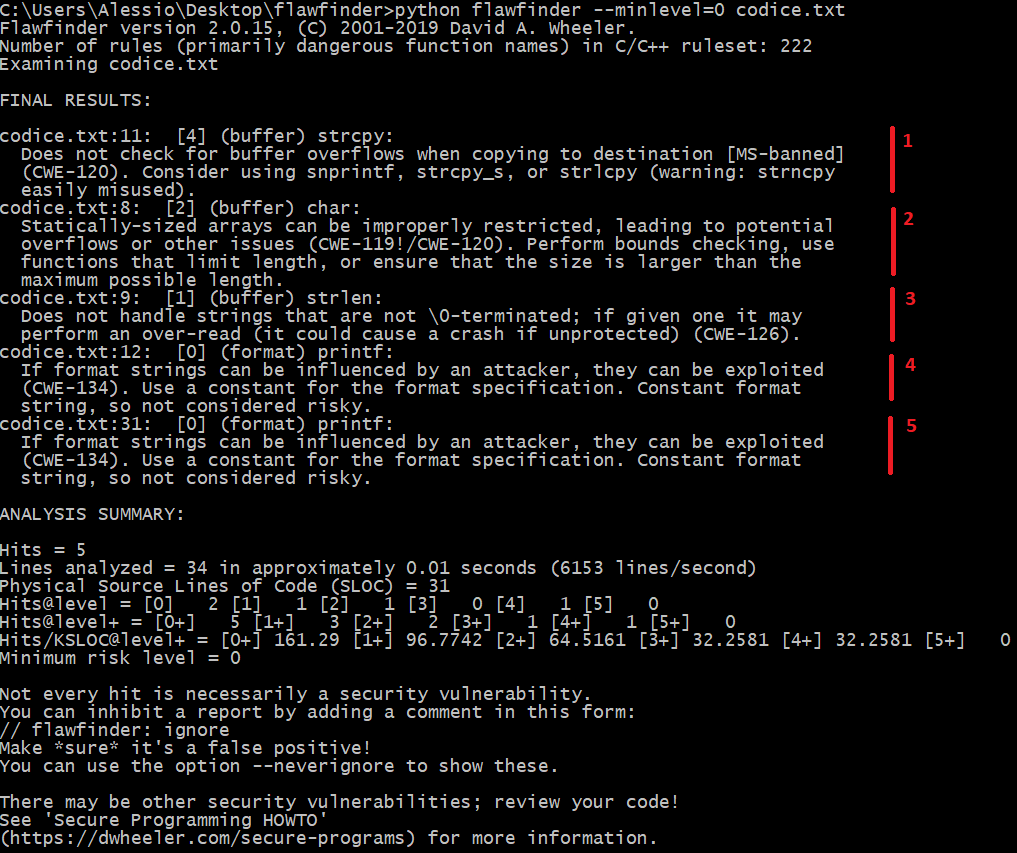
\includegraphics[scale=0.6]{output}
\newline

Utilizzando il parametro --minlevel=0 (in modo da segnalare anche gli avvertimenti con livello di rischio pari a 0) il programma segnala 5 hit:
\begin{enumerate}
\item{Il primo hit si trova sulla riga 11, ha un livello di rischio pari a 4 ed ha a che fare con la funzione strcpy(). La funzione strcpy(char *dest, const char *src) viene utilizzata per copiare la stringa di origine nella stringa di destinazione. Ritorna un puntatore alla stringa di destinazione. La funzione strcpy ha alcuni problemi infatti non controlla se il buffer di destinazione è abbastanza grande e quindi si \textbf{potrebbe} verificare buffer overrun. In particolare, se la stringa di destinazione non è abbastanza grande per memorizzare la stringa di origine, il comportamento di strcpy() non è specificato o definito. \newline
Si possono adottare diverse soluzioni: una prevedere di effettuare dei controlli direttamente sul buffer oppure si può sostituire tale funzione con altre nelle quali viene specificato il numero di caratteri da gestire come, ad esempio, strncpy(). La funzione char *strncpy(char *dest, const char *src, size\_t n ) è simile alla funzione strcpy(), tranne per il fatto che vengono copiati al massimo n byte di src. Se non è presente alcun carattere NULL tra i primi n caratteri di src, la stringa inserita in dest non terminerà con NULL. Se la lunghezza di src è inferiore a n, strncpy() scrive caratteri NULL aggiuntivi in dest per garantire che venga scritto un totale di n caratteri. Se non c'è un carattere null tra i primi n caratteri di src, la stringa inserita in dest non avrà terminazione null. Quindi strncpy() non garantisce che la stringa di destinazione terminerà con NULL e questo potrebbe portare ad un segmentation fault. Bisogna quindi aggiungere un controllo per assicurarsi che la stringa abbia il carattere terminatore;}
\item{Il secondo hit si trova sulla riga 8 ed ha un livello di rischio pari a 2. Questo avvertimento segnala la presenza di un array di dimensioni statiche. Il problema con questo tipo di array è che possono essere limitati in maniera impropria portando a potenziali overflow. In questo caso, probabilmente si tratta di un falso positivo e, in ogni caso, per risolvere questo problema sarebbe opportuno aggiungere alcuni controlli sulla lunghezza e assicurarsi che grandezza dell'array sia maggiore della lunghezza massima possibile;}
\item{Il terzo hit si trova nella riga 9, ha un livello di rischio pari a 1 ed ha a che fare con la funzione strlen(). Questo avvertimento segnala semplicemente di fare attenzione al comportamento della funzione strlen() che calcola la lunghezza di una stringa escluso il carattere terminatore. Inoltre continua a leggere la stringa finchè non trova il carattere terminatore e, se non presente, potrebbe leggere caratteri che non fanno parte della stringa in considerazione (si effettua quindi over-read). Sarebbe opportuno assicurarsi che la stringa di cui calcolare la lunghezza abbia il carattere terminatore;}
\item{Il quarto hit si trova sulla riga 12, ha un livello di rischio pari a 0 ed ha a che fare con la funzione printf(). Questo avvertimento segnala che la funzione printf() può essere vulnerabile a vari attacchi che sfruttano il formato della stringa. Ad esempio, senza i dovuti controlli, il comando printf("\%s\%s\%s\%s\%s\%s\%s\%s\%s\%s\%s\%s") potrebbe portare ad un crash del programma mentre il comando printf ("\%08x \%08x \%08x \%08x \%08x") potrebbe permettere di visualizzare lo stack. Ulteriori informazioni disponibili \href{https://web.ecs.syr.edu/~wedu/Teaching/cis643/LectureNotes_New/Format_String.pdf}{qui}. Una possibile contromisura a questo tipo di problemi potrebbe essere la randomizzazione degli indirizzi che rende difficile per gli aggressori scoprire quale indirizzo vogliono leggere/scrivere oppure metodi per la validazione dell'input;}
\item{Il quarto hit si trova sulla riga 31, ha un livello di rischio pari a 0 ed ha a che fare con la funzione printf(). Si tratta dello stesso avvertimento del punto precedente.}
\end{enumerate}

\subsection{Ulteriori errori}
\label{sec:err}
Un ulteriore errore non individuato da Flawfinder si trova nella funzione main, nel seguente blocco di codice:
\begin{lstlisting}
	...
	int i[10];
	int j = 0;
	while (j < 10000)
	{
		i[j] = 5; //RIGA 27			 
		++j;
	}
	...
\end{lstlisting}
Come si può facilmente notare, viene istanziato un array i di grandezza 10. Successivamente si effettua un ciclo while il cui corpo viene reiterato finchè j$<$10000. Si noti che nella riga 27 si verifica un segmentation fault perchè si sta tentando di accedere ad una posizione di memoria non istanziata. Ad esempio, se j=15 allora i[15]=5 ma la dimensione dell'array i è 10! \newline
Questo problema si può risolvere semplicemente aggiustando la grandezza dell'array o il numero di iterazioni del ciclo while. Ad esempio, si potrebbe modificare while(j$<$10000) con while(j$<$10). La scelta definitiva verrà data dal programmatore in base a cosa vuole fare all'interno del programma.

\newpage

\subsection{Correzione del codice}
In base alle considerazioni fatte nelle precedenti sezioni, sono state effettuate alcune modifiche al codice:
\newline

\begin{lstlisting}
#include <stdio.h>
#include <string.h>

#define	MAXSIZE	40
void
test(char *str)
{
	char buf[MAXSIZE+1] = {0};
	int i = strnlen(str, MAXSIZE+1);
	if(i > MAXSIZE) return;
	else
	    strncpy(buf, str, MAXSIZE);
	    printf("result: %s\n", buf);
}


int
main(int argc, char **argv)
{
	char *userstr;
	if(argc > 1) {
		userstr = argv[1];
		test(userstr);
	}
	int i[10];
	int j = 0;
	while (j < 10)
	{
		i[j] = 5;
		++j;
	}
	for (j = 0; j < sizeof i / sizeof i[0]; ++j)
		printf("Value = %d\n", i[j]);
	return 0;
}
\end{lstlisting} \newpage
Si \textbf{suppone} che MAXSIZE sia la lunghezza massima della stringa \textbf{senza carattere terminatore}. Prima di tutto si istanzia un array \textbf{nullo} buf di dimensione MAXSIZE+1 dove l'ultima posizione è riservata esclusivamente al carattere terminatore. Successivamente si controlla la lunghezza della stringa con la funzione strnlen(const char * s, size\_t maxlen). Tale funzione restituisce strlen(s), se è minore di maxlen, o maxlen se non c'è alcun carattere \textbackslash0 tra i primi caratteri maxlen puntati da s. In questa maniera si può controllare con facilità se la stringa in input ha il carattere terminatore o è lunga al più n caratteri. Si controlla se l'output della funzione strnlen() è maggiore del valore MAXSIZE, in tal caso significa o che la stringa non ha carattere terminatore (si effettua overrun) oppure la stringa ha il carattere terminatore ma è più lunga di MAXSIZE. In tal caso si effettua un return, altrimenti si copiano al più MAXSIZE caratteri di str in buf (buf[40] sarà sempre e in ogni caso\textbackslash0). \newline
Inoltre, viene risolto anche il problema di segmentation fault nella funzione main già spiegato nella sottosezione \hyperref[sec:err]{"ulteriori errori"}. \newline
Presentando nuovamente il codice corretto a Flawfinder, vengono comunque segnalate alcune vulnerabilità ma molto probabilmente si tratta di falsi positivi dati dal fatto che Flawfinder non utilizza informazioni sul flusso di controllo e sul flusso dei dati. \newline \newline
Nota: Nella seguente soluzione vengono effettuate alcune correzioni nonostante non siano propriamente necessarie. Ad esempio, si va ad effettuare un controllo sul fatto che stringa abbia un carattere terminatore ma siamo già certi di questa cosa perchè è un argomento della funzione main (gli argomenti del main hanno tutti il carattere terminatore). Inoltre si ha la certezza del fatto che tale stringa (senza carattere terminatore) sia lunga al più MAXSIZE in quanto effettuiamo un controllo preventivo prima di copiarla nel buffer di destinazione e quindi la sostituzione di strcpy() con strncpy() diventa quasi superflua. Le varie sostituzioni presenti nella correzione sono state inserite come un ulteriore metodo di prevenzione e per mostrare che esistono funzioni più sicure di altre (es. strncpy()).


\subsection{Test del codice}
Una volta effettuate tutte le correzioni, il codice viene eseguito con successo non presentando più gli errori presenti nel codice iniziale. Sono stati eseguiti due test di prova:
\begin{enumerate}
\item{Nel primo test è stato dato in input il valore "testtesttesttesttesttesttesttesttesttest". Si noti che la dimensione dell'input è minore della dimensione del buffer di destinazione. La lunghezza della stringa è 40 (41 con il carattere terminatore) e quindi viene copiata correttamente all'interno del buffer di destinazione (viene eseguito il codice all'interno dell'if). Si ricorda che la lunghezza del buffer è uguale a MAXSIZE+1, dove MAXSIZE=40 quindi verranno copiati al pià 40 caratteri della stringa e l'ultimo carattere in buf sarà per forza \textbackslash0. Viene eseguito anche il resto del codice nella funzione main che non fa altro che stampare i valori dell'array i: \newline 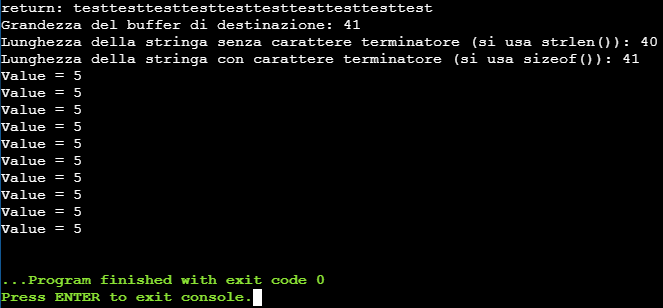
\includegraphics[scale=0.8]{test1} }
\item{Nel secondo test è stato dato in input il valore "testtesttesttesttesttesttesttesttest1". Si noti che la dimensione dell'input è maggiore della dimensione del buffer di destinazione. La lunghezza della stringa è 41 (42 con il carattere terminatore) e quindi non viene copiata all'interno del buffer di destinazione (non viene eseguito il codice all'interno dell'if in quanto i=41 \textgreater MAXSIZE=40). Viene comunque eseguito il resto del codice nella funzione main che non fa altro che stampare i valori dell'array i: \newline 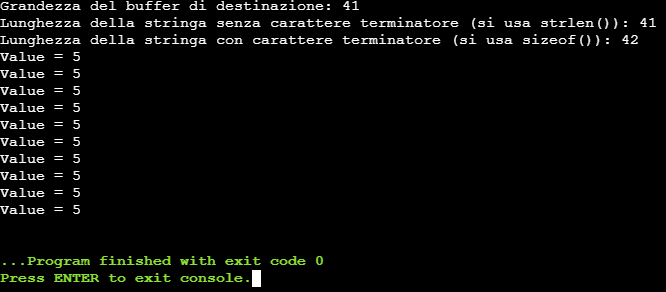
\includegraphics[scale=0.8]{test2}}
\end{enumerate}

\section{Risorse utilizzate}
Nello svolgimento di questo progetto sono state utilizzate le seguenti risorse:
\begin{itemize}
\item{\href{https://dwheeler.com/flawfinder/}{FlawFinder}}
\item{\href{https://www.latex-project.org/}{\LaTeX}}
\item{\href{https://www.onlinegdb.com/}{Online C Compiler}}
\end{itemize}


\end{document}